\documentclass{article}
\usepackage[a4paper, left=1in, right=1in, top=1in, bottom=1in]{geometry}
\usepackage{amsmath}
\usepackage{amssymb}
\usepackage{physics}
\usepackage{graphicx}

\title{Mini-DFS report}
\author{Mingkun Huang}
\date{\today}

\begin{document}
\maketitle

\section{System Structure}
Mini-DFS is running through a process. In this process, the name server and data servers are different threads.
The system structure is shown in figure~\ref{fig:dfs}.

\begin{figure}[tbh]
    \centering
    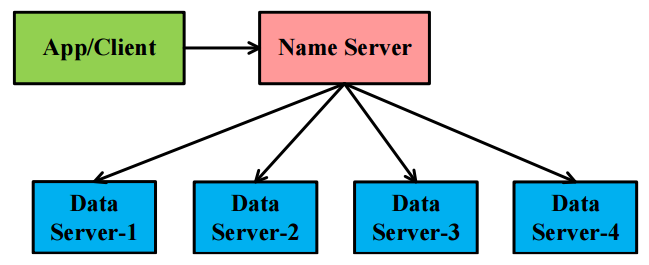
\includegraphics[scale=.5]{project4_pic1}
    \caption{System structure}
    \label{fig:dfs}
\end{figure}

\section{Basic Functions}
\begin{itemize}
    \item Read/write a file
        \begin{itemize}
            \item Upload a file: upload success and return the ID of the file
            \item Read the location of a file based on the file ID and the offset
        \end{itemize}
    \item File striping
        \begin{itemize}
            \item Slicing a file into several chunks
            \item Each chunk is 2MB
            \item Uniform distribution of these chunks among four data servers
        \end{itemize}
    \item Replication
        \begin{itemize}
            \item Each chunk has three replications
            \item Replicas are distributed in different data servers
        \end{itemize}
    \item Directory management
        \begin{itemize}
            \item Write a file in a given directory
            \item Access a file via "directory + file name"
        \end{itemize}    
\end{itemize}

\section{Details of Each Component}
\subsection{Name Server}
\begin{itemize}
    \item List file tree
    \item List the relationships between file and chunks
    \item List the relationships between replicas and data servers
    \item Data server management
\end{itemize}

\subsection{Data Server}
\begin{itemize}
    \item Read/Write a local chunk
    \item Write a chunk via a local directory path
\end{itemize}

\subsection{Client}
\begin{itemize}
    \item Provide read/write interfaces of a file
\end{itemize}

\section{System Design}
The whole system flowchart is shown in figure~\ref{fig:flowchart}.
\begin{figure}[tbh]
    \centering
    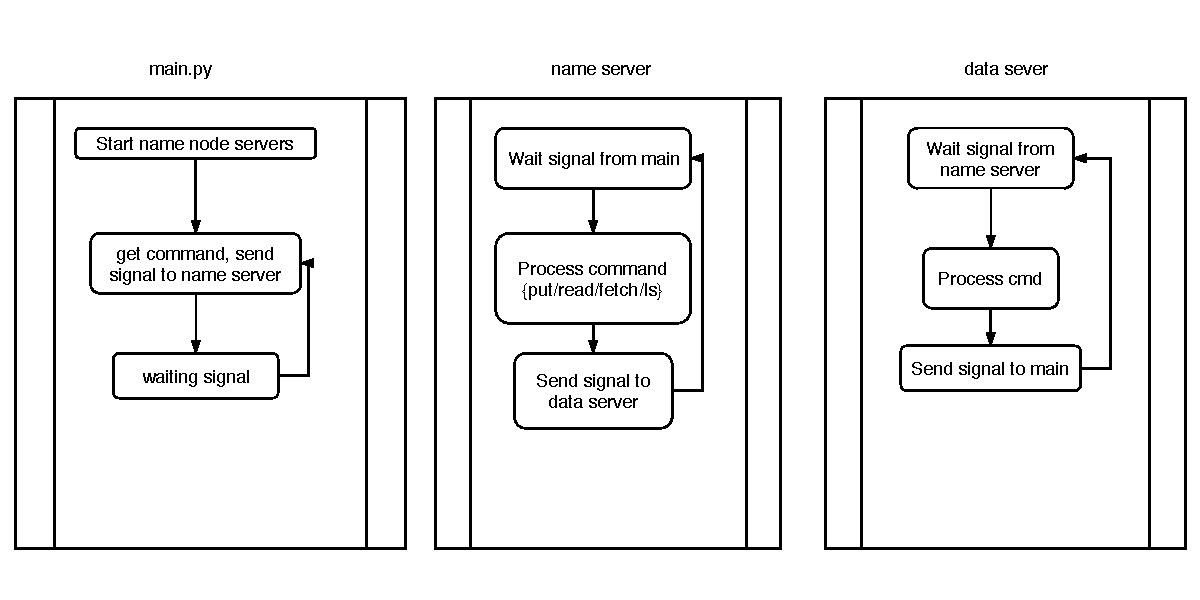
\includegraphics[scale=.8]{minidfs}
    \caption{System flowchart}
    \label{fig:flowchart}
\end{figure}

\subsection{Data Structure}
\begin{itemize}
    \item Global events:
        \begin{itemize}
            \item name\_event: Name server wait for this event, send by main.py. 
            \item data\_events: 4 data servers, 4 events. Name server send this signal to control data server.
            \item main\_event: wait for dataserver in main.py
            \item read\_event: data server send this signal to main.py once success read, and name server send this signal to main.py for some error.
            \item ls\_event: name server list files, then send this signal to main.py
        \end{itemize}
    \item Name server:
        \begin{itemize}
            \item id\_chunk\_map: map file id to chunks, eg. {0: ['0-part-0', '0-part1'], 1: ['1-part-0', '1-part-1']}
            \item id\_file\_map: map file id to file info, eg. {0: ('file1', size1), 1: ('file2', size2)}
            \item chunk\_server\_map: map chunk to its replications, eg. {'0-part-0': [0, 1, 2, 3]}
            \item last\_file\_id: the maximum file id
        \end{itemize}
\end{itemize}

\subsection{Commands Effects}
\begin{itemize}
    \item Put\\
        1. get file id, split file size into chunks\\
        2. mapping file id to chunks, update id\_chunk\_map\\
        3. mapping file id to file info, update id\_file\_map\\
        4. add chunks to each data server, update server\_chunk\_map
    \item Read\\
        1. get file id and offset count \\
        2. calculate start chunk \\
        3. send signal to data server 
\end{itemize}

\section{Instructions}
\begin{itemize}
    \item ls: list all files in DFS.
    \item ls2: list file tree.
    \item mkdir $<$file\_dir$>$: make dir in DFS.
    \item put $<$source\_file\_path$>$: upload local file to DFS, and return file id.
    \item put2 $<$source\_file\_path$>$ $<$put\_savepath$>$: upload local file to DFS, specify server dir, and return file id.
    \item read $<$file\_id$>$ $<$offset$>$ $<$count$>$: read from DFS using file id.
    \item read2 $<$file\_dir$>$ $<$offset$>$ $<$count$>$: read from DFS using file path.
    \item fetch $<$file\_id$>$ $<$save\_path$>$: download file from DFS using file id, save file to local path.
    \item fetch2 $<$file\_dir$>$ $<$save\_path$>$: download file from DFS using file path, save file to local path.
\end{itemize}

\end{document}